\chapter{Course Organization}

\section{About the Lecturer}

\begin{minipage}{0.2\linewidth}
	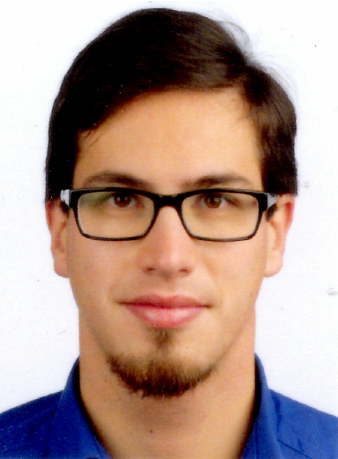
\includegraphics[width=0.8\linewidth]{../chapter00/Philipp.jpg}
\end{minipage}
\hfill
\begin{minipage}{0.75\linewidth}
	Philipp Le
	
	philipp.le@st.ovgu.de
\end{minipage}

\vspace{1em}

\underline{Academic CV:}

\begin{tabular}{p{0.2\linewidth}p{0.7\linewidth}}
	2011 -- 2015 & \makecell[l]{\textbf{B.\,Sc.} in Electrical Engineering and Information Technology,\\ Otto-von-Guericke-University Magdeburg} \\[1.5em]
	2016 & Exchange student, TU Tampere, Finland\\[0.5em]
	2015 -- 2019 & \makecell[l]{\textbf{M.\,Sc.} in Electrical Engineering and Information Technology,\\ Specialization: Communication Technology and Microwave Engineering\\ Otto-von-Guericke-University Magdeburg} \\[0.5em]
\end{tabular}

\vspace{2em}

\underline{Current occupation:}

\begin{quote}
	Since 2015: Hardware and Firmware Developer at
	
	\textbf{metraTec GmbH, Magdeburg}
	
	located in the Wissenschaftshafen.
	
	\vspace{1em}
	
	Main topics:
	\begin{itemize}
		\item Low power radio devices, IoT
		\item Radio localization
		\item Microwave engineering
	\end{itemize}
\end{quote}


\section{Course Overview}

\textit{Subject to change}

Facts on the course:
\begin{itemize}
	\item Duration: 1 semester (summer semester), 14 weeks
	\item E-Learning webpage: \url{https://elearning.ovgu.de/course/view.php?id=7849}
	\item Course material is published on the E-Learning webpage:
	\begin{itemize}
		\item Lecture notes
		\item Exercise sheets
		\item Supplementary material
	\end{itemize}
	\item Work load: 150 h (1 h = 45 minutes), yielding \textbf{5 ECTS}
	\begin{itemize}
		\item 42 h of attendance
		\item 108 h autonomous work
	\end{itemize}
	\item The research report mentioned in the module description is neglected in this semester, due to a lack of time.
	\item Written exam (120 minutes)
	\item Attending lectures or exercises not mandatory, but recommended.
\end{itemize}

Dates:
\begin{itemize}
	\item Every week: \textbf{Thursdays at 9:15 -- 10:45 (a.m.)}
	\begin{itemize}
		\item Exception: 2020-05-21 is a public holiday, no lecture! We will meet on 2020-05-19 at 15:15 -- 16:45 instead.
	\end{itemize}
	\item Additional date if necessary: Tuesdays at 15:15 -- 16:45. Will be explicitly announced on E-Learning.
	\item We will use a videoconferencing tool for our meetings. I will announce details in the E-Learning.
\end{itemize}


\section{Lecture Details}

Study organization:
\begin{itemize}
	\item You are required to elaborate major parts of the course in \underline{self-study}.
	\item The chapters of the lecture notes will be published in the E-Learning on weekly basis.
	\item Please go through the lecture notes \underline{on your own}.
	\item The lecture will be held in form of a \textbf{consultation} where we will discuss the main topics of the chapter.
	\item A pre-requisite is that you have read the lecture notes beforehand.
\end{itemize}

Remarks on the lecture notes:
\begin{itemize}
	\item The lecture notes shall give you a good foundation for your self-studies. It contains the relevant course content.
	\item If you find mistakes, don't hesitate to communicate them to me. I'm currently writing the lecture notes in nightshifts, which may lead to mistakes slipping through. ;)
\end{itemize}


\section{Exercise Details}

Goal of the exercises:
\begin{itemize}
	\item Strengthening your knowledge that you have gained in the lecture.
	\item Bringing your knowledge into action.
	\item Learning how to deal with the course material and further sources.
	\item Getting used to the nature of questions which will be asked in the exam. However, exam questions will be different.
\end{itemize}

Exercise in self-study:
\begin{itemize}
	\item Exercise sheets will be published in the E-Learning.
	\item Solve them individually or \underline{in groups}.
	\item You may ask for clarification of an exercise task at any time.
	\item \underline{You are required to put reasonable effort in solving the exercise.} This comprises referring to the lecture notes, supplementary material or other sources including the library and the internet.
	\item If you get stuck, you can contact me. I will give hints. Please be sure that you have put reasonable effort in solving beforehand.
\end{itemize}

Optional returning of solutions:
\begin{itemize}
	\item You may voluntarily return your solutions to me via E-Learning. This is not mandatory.
	\item If you wish to return your solutions, please do so within \underline{two weeks} after their publication.
	\item I will skim your solutions. Unfortunately, it is not possible for me to provide you individual corrections, as I'm lecturing besides my full time job.
	\item Of course, you may ask questions along with returning the exercises, preferably via e-mail or in the E-Learning.
	\item If I see major issues, we will discuss them together. I will integrate this into the \textbf{consultation}. The Tuesday date may be optionally used, if necessary.
	\item However, if nobody sends me a solution, we cannot discuss anything.
\end{itemize}

Please be patient if I don't answer your requests immediately. I'm giving my best to respond as soon as possible. But, I'm having a full time job which is also consuming time. :)


\section{Homework}

Your \underline{weekly} homework comprises:
\begin{itemize}
	\item Going through the lecture notes and understand its contents.
	\item If necessary, consulting further sources (library, internet) is strongly recommended.
	\item Solving the exercises.
\end{itemize}


\section{Exam Details}

\textit{All information are subject to change. There will be an announcement with details on the exam at the end of the course.}

\begin{itemize}
	\item Written exam
	\item Date: will be announced by the examination office
	\item Duration: 120 minutes
	\item Information on tools allowed will be announced at the end of the lectures.
	\item The exam covers the complete course content (all chapters, all exercise sheets).
	\item The exam questions call for different levels of skills:
	\begin{itemize}
		\item Memorized knowledge
		\item Bringing knowledge into practise
		\item Creatively deriving solutions from the knowledge
	\end{itemize}
	\item Grading scale guideline:
	\begin{itemize}
		\item 1.0 (very good): Exam performance is outstanding and goes beyond the requirements.
		\item 2.0 (good): Exam performance fulfils overall requirements.
		\item 3.0 (satisfactory): Requirements are fulfilled in general. There are minor deficiencies.
		\item 4.0 (pass): Exam performance meets the requirements, but shows major deficiencies.
		\item 5.0 (fail): Exam performance is insufficient.
	\end{itemize}
	\item Individual work. Cheating will result in a 5.0 grade (failed).
\end{itemize}


\section{Feedback Poll}

A feedback poll is required by the universities regulations for quality assurance in the teaching. Furthermore, the poll will help me to improve this course.

\textbf{So I kindly ask you to participate in the poll.}

\begin{itemize}
	\item The poll will be at the end of the course.
	\item There is an online form.
	\item The poll is completely anonymous.
	\item Participating is voluntary for you.
	\item Of course, the poll will not affect the grading. It is anonymous.
\end{itemize}
